\documentclass[PhD-Yoann-Dupont.tex]{subfiles}
\begin{document}

ESSEX (Expert System Semantic Engine eXtended server) est l'outil utilisé par Expert System afin d'effectuer l'analyse syntaxique et sémantique d'un document, il est au c\oe ur de l'ensemble des outils d'Expert System.

L'architecture générale d'ESSEX est donnée dans la figure\ \ref{fig:essex-architecture}. pour effectuer ses analyses, il recourt à une resource sémantique, le Sensigrafo, ainsi qu'à un désambiguisateur, le \emph{Semantic Disambiguator}.

Le Sensigrafo est un graphe sémantique dans lequel sont organisés des \emph{lemmes} regroupés dans diverses classes appelées \emph{syncons}. Chaque \emph{syncons} a des attributs, comme sa fréquence où son domaine, qui permettent au système de désambiguisation de décider quel syncon attribuer à chaque token étant donné le contexte global. Ces \emph{syncons} sont reliés entre eux par des liens comme l'hyperonymie et l'hyponymie, la partition et l'ensemble (un pétale est une partie d'une fleur, une fleur contient un pétale, une tige, etc.).

Le \emph{Semantic Disambiguator} effectue une analyse du texte en quatre phases : l'analyse lexicale, l'analyse grammaticale, l'analyse syntaxique et l'analyse sémantique. L'analyse lexicale effectue une annotation sytnaxique au niveau des tokens (appelés \emph{atomes}). L'analyse grammaticale regroupe les tokens ainsi analysés dans une \emph{forme} (par exemple, le nom complet d'une personne a plusieurs tokens mais une seule forme). L'analyse syntaxique, quant à elle, regroupe les formes selon des \emph{chunks} (groupe nominal, noyaux verbal) et des \emph{clauses}, en plus de retrouver les divers \emph{sujets}, \emph{prédicats} et \emph{objets}. L'ensemble de cette analyse syntaxique est représentée dans la figure \ref{fig:cogito-syntactic-analysis}.

\begin{figure}[ht!]
\centering
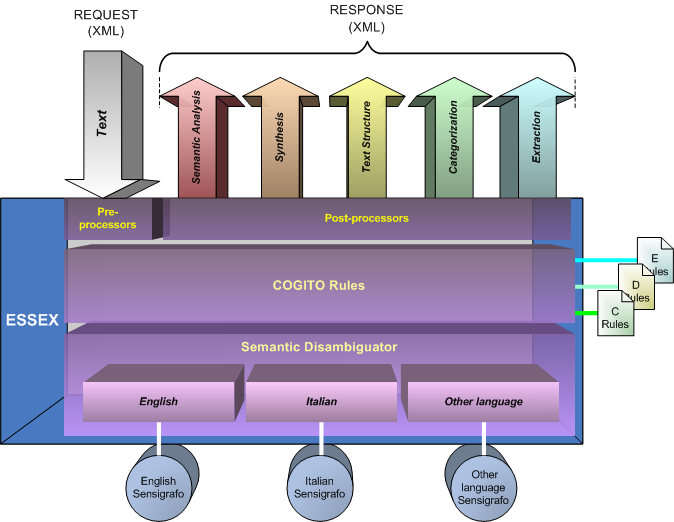
\includegraphics[scale=0.4]{images/ExpertSystem/ESSEX-Architecture}
\caption{architecture d'ESSEX}
\label{fig:essex-architecture}
\end{figure}

\begin{figure}[ht!]
\centering
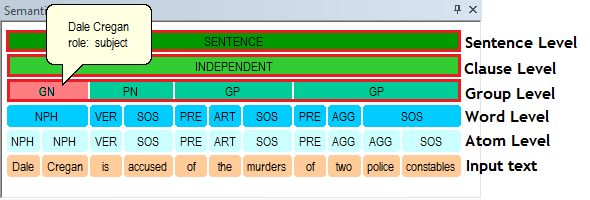
\includegraphics[scale=0.7]{images/ExpertSystem/disambiguation_html_21066960}
\caption{analyse syntaxique servant de base à ESSEX}
\label{fig:cogito-syntactic-analysis}
\end{figure}

L'analyse au sémantique est la phase où sont extraites les entités nommées. Dans cette phase, lorsque le système rencontre un élément inconnu, le système effectue une analyse du contexte afin de lier cet élément à un \emph{syncon} dans le Sensigrafo, ce \emph{syncon} déterminera alors l'entité à laquelle est ratachée un élément. Par exemple : ``deux heures du matin'' sera relié au \emph{syncon} représentant l'heure comme unité de temps.

\end{document}